\chapter{Evaluation}
\label{chap:evaluation}
We have divided the evaluation of our system into 2 important sections. The selection interface
deals with a more qualitative topic, since its performance is dependent on how easy users find 
selecting items for extraction. For this component of the system, we conducted a human
evaluation on the qualitative performance of the system. In the second section, we will describe
the evaluation of the machine learning technique we have used, and how well this performs when
attempting to extract data from a webpage after a layout change.

In summary, these are the questions we hope to answer with our evaluation:
\begin{enumerate}
	\item What is the current awareness level of Web Information Extraction?
	\item How easy is it to do various web IE tasks using our system?
	\item How well does the robust wrapper perform on modified web page layouts?
\end{enumerate}



\section{Human evaluation of Selection Interface}

For the evaluation of this part of the system, a group of 30 students were paid to do a simple 30
minute evaluation of the system. A simple tutorial was given to each of the students, and once
completed, a simple extraction task from the bookdepository.co.uk website was to be carried out.
Lastly, the students were asked to fill out a questionnaire on the following aspects of the
system: Ease of installation of the bookmarklet, the ease of item selection, and the ease with
which they could view the extracted items. The full content of the entire survey can be found in
the appendix, along with the survey results.

The students were from various tertiary institutions in Singapore, and were given a small sum of
money for their time.

\input userstudy.tex

\subsection{Analysis}
The participants were asked to rank the ease of use for the installation of the bookmarklet on
a scale of 1 to 5, with 1 being ``Really easy" and 5 being ``Really difficult".
 On the average, the score was 1.63 The installation procedure was meant to
be simple and easy: Dragging the button from the page to the toolbar. However, some of the 
participants had an issue with this since some browsers, for example Chrome, do not show their
toolbars by default. 
\begin{quote}
\textit{Installation was hassle-free. No need to restart browser (like in the case of plugins)}
\end{quote}
\begin{quote}
\textit{
I think that should be the most simple way to install a bookmarklet. 
I think you should consider the case when the bookmark toolbar is hidden,
and if it's possible, show a tutorial video for beginner.}
\end{quote}

On the intuitiveness of the selection procedure, the average score was 2.27
Some of the participants found the interface for modifying existing labels confusing,
while some had issues when trying to select elements ``behind" its child elements.
\begin{quote}
\textit{
When the bookmarket is initially started, it does not intuitively guide the user as
to how they are to go about choosing the elements they want from the page. Editing existing
labels can be confusing.}
\end{quote}
76.67\% of the participants found the visual feedback for the selection procedure useful
in understanding what the extractor would be extracting. 

Viewing the extracted data seemed to be a problem for many of the participants. The average
score given for the ease of viewing extracted data was at 2.73 This may be due to the way
in which the page is updated after the data has been extracted and inserted into the database.

\begin{quote}
\textit{
Nothing seems to have changed when I click ``extract" a couple of times. 
Maybe include a ``estimated time left" bar or progress bar?
At least something to indicate whether the extracting is completed or
still in progress or something went wrong and nothing was registered.}
\end{quote}

In general, we find that the selection interface has been successful in aiding
the process of annotation by giving visual feedback. However, there were still
glaring issues in the interface used for viewing the extracted data. We intend to
correct these cosmetic problems in the next version of the system.

\section{Machine Learning evaluation}
 We want to be able to extract the same content from pages which have had a layout change. So our
 evaluation method involves attempting to extract data after a layout change by training a
 classifier for the previous.
 
 For this evaluation, we have selected the archived pages of Digg from Web Archives. This is
 due to the fact that Digg has a front page with structured entries, very much like a search
 entry. Also, Digg has gone through several layout changes over the years, making it an excellent
 candidate to perform this experiment on.
\subsection{Methodology}
	Since our system only uses the learnt models when the layout of the page changes (which is 
detected when the XPath does not retrieve any items), we have restricted the evaluation of 
the learnt models between layout changes.

	We use old pages from web.archive.org to simulate pages that have not
undergone a layout change. To define a layout change, we use the tree-edit distance \cite{Zhang1989} between two pages as
a simple metric. In order to find layout changes within the list of pages we retrieved from Web
Archive, we took the tree-edit distance of the DOM tree between every pair of consecutive pages.
The graph of these values is shown in Figure \ref{fig:scoregraph}.

\begin{figure}[htbp]
\centering
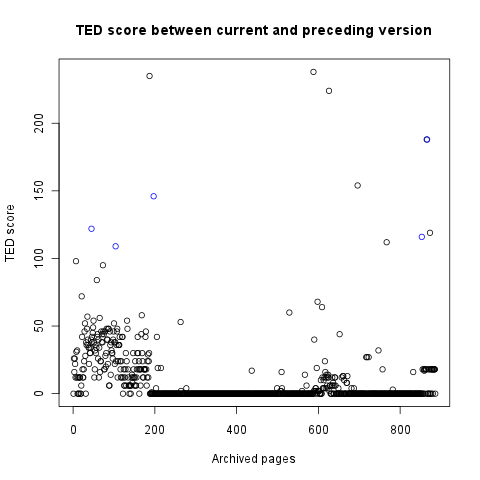
\includegraphics[scale=0.6]{scoregraph.png} 
\caption{Graph of Tree Edit Distance between adjacent pages}
\label{fig:scoregraph}
\end{figure}

	The spikes visible in the graph were signals of a high tree-edit distance between the pairs
of pages, and signals some sort of layout change. What we are looking for, however, are changes
in which the XPaths fail to work. For each of the labels we are hoping to extract, we check
if the application of the XPath yields any resulting DOM nodes. If they do not, the page was
considered a layout change, and the pages prior the change were randomly sampled for 20 instances
for learning. On the graph, these nodes are shown in blue.

	 We created 5 sets of 20 pages from the pages retrieved from web
then trained the classifier on each of these. The test results were then compared to the data
extracted if an XPath was created manually for each of these sets.
 
 
\subsection{Analysis}
Before we present our results, we compare our results to the performance
of the robust wrappers in \cite{Dalvi2009} by estimating our
robustness performance if we performed the same experiment.

Their work aims to produce robust XPath wrappers resilient to changes 
in layout by measuring the probability of different DOM edits in past pages
from the Web Archive\footnote{\url{http://web.archive.org}}

We differ from their evaluation methods in the choosing of test corpus. In their testing
set, they have used 3 pages for learning, while testing their wrapper on 15 pages,
each 2 months apart, without taking into account if the pages have a change in layout.

	We intend to compare our performance by estimating how well our classification method will do, given the same
method of evaluation.
\subsubsection{Estimation method}
Due to the popularity of Digg compared to IMDB, the page has been indexed more by Web Archives.
In our data set, we have 895 pages downloaded from IMDB. From this, we extracted 15 snapshots
with 2 month intervals. We then calculated the accuracy of the extractor in the following manner:

\begin{figure}[htbp]
\singlespacing
	\begin{algorithm}[H]
	\caption{Calculating performance of a wrapper over an interval}
	\begin{algorithmic}[1]
		\IF{$D^{(t)} \to D^{(t+1)}$ has layout change}
			\STATE $M \leftarrow$ models trained using batch corresponding to $D^{(t)}$
			\STATE $w \leftarrow$ models with $F_1$ score above $\alpha$ in $M$
			\RETURN $\frac{w}{|M|}$
		\ELSE
			\RETURN 100\% accuracy (this is the way we have defined the different datasets.)
		\ENDIF
	\end{algorithmic}
	\end{algorithm}
\label{fig:evalmeth}
\end{figure}
It is unclear from the paper what XPath is defined as working, so we assume that
the XPath fails when it returns no corresponding element. In our learned model,
our models do not generally work completely (retrieving a 100\% of all items),
nor do they fail completely. Therefore, in order to estimate a result, we use 
a threshold $\alpha$ on the $F_1$ measure of the model. If $F_1 > \alpha$,
then we consider the model to be `working'.


We have set $\alpha = 90\%$ as a threshold for our models. 
Since for our dataset the number of extracted items are the same (15) for each page,
we have simply calculated the percentage of the models that would work.

\begin{table}
\centering
\small
\singlespacing
\begin{tabular}{|c|l|c|}
\hline
	Interval			  & Change state & Robustness\\
\hline
	$D^{(1)} \to D^{(2)}$ & Change		& 75\%\\
	$D^{(2)} \to D^{(3)}$ & No Change 	& 100\%\\
	$D^{(3)} \to D^{(4)}$ & Change 		& 0\%\\
	$D^{(4)} \to D^{(5)}$ & No Change 	& 100\%\\
	$D^{(5)} \to D^{(6)}$ & No Change 	& 100\%\\
	$D^{(6)} \to D^{(7)}$ & No Change 	& 100\%\\
	$D^{(7)} \to D^{(8)}$ & No Change 	& 100\%\\
	$D^{(8)} \to D^{(9)}$ & No Change 	& 100\%\\
	$D^{(9)} \to D^{(10)}$ & No Change 	& 100\%\\
	$D^{(10)} \to D^{(11)}$ & No Change 	& 100\%\\
	$D^{(11)} \to D^{(12)}$ & No Change 	& 100\%\\
	$D^{(12)} \to D^{(13)}$ & No Change 	& 100\%\\
	$D^{(13)} \to D^{(14)}$ & No Change 	& 100\%\\
	$D^{(14)} \to D^{(15)}$ & No Change 	& 100\%\\
\hline 
\end{tabular}
\caption{$D^{(t)}$ intervals and their corresponding layout changes}
\label{tab:dalvicomp}
\end{table}

Using the numbers in Table \ref{tab:dalvicomp} , we arrive at an overall precision of 91.07\%. This result
is significantly better than the robust XPath wrappers generated using their method. However,
it should be noted that this result is estimated, and the dataset used in this experiment may
be drastically different from that of the IMDB archive. Also, this method is slightly more forgiving
since the model is still considered ``working" even though it does not have a 100\% precision
and recall.

We have also performed a stricter form of evaluation using our data set that uses pages
grouped by layout changes. This means the model is used only after a drastic layout change
that causes the XPath to no longer work.

\begin{table}
\centering
\small
\singlespacing
\begin{tabular}{|c|l|c|c|c|c|c|c|c|c|c|}
\hline
Batch	&Label	&TP	&FP	&FN	&TN	&	&Precision	&Recall& $F_1$ & Accuracy\\
\hline
\input groupeddigg.tex
\hline 
\end{tabular}
\caption{Learnt model evaluation results for digg.com}
\label{tab:mlevalres}
\end{table}


	The results of our method of evaluation is shown in Table \ref{tab:mlevalres}.
Aside from the first layout change, the other layout changes sometimes do not extract anything
at all. This is probably due to the fact that Digg underwent a significant layout change that
rearranged the locations of the individual items within each entry, rendering the model learnt
useless. Also, some of the labels, like the article poster's username, are harder to learn
than others, since not many defining features could be extracted. Of the results retrieved,
only TITLE, AUTHOR and SUMMARY for Batch 0. The learner seems to have a problem dealing with
elements with short text content. Also, the poor performance is partly by 
the classifier selecting elements that are either the direct child or parent of the target node.
This is due to the fact that the content in the tags are almost the same, since the wrongly
selected tag may either be an immediate ancestor or descendant of the wanted node. 
At the very least however, the data collected suggests that our approach achieves comparable
results with the state-of-the-art.